\chapter{Result}
The result from the multiple runs we have gotten is as shown in the different figures. Figure \ref{fig:smallResult} shows the spread and coverage from the simulation of the small graph. As we can see, the four different algorithm had little difference. The y-akses shows us the average coverage after 50 runs, and the x-akses gives us how many seed node was selected. We can see from figure \ref{fig:smallResult}, figure \ref{fig:mediumResult} and figure \ref{largeResult} that the resulted coverage was around 0.3-0.45. The smaller graph would result in a smaller spread, while larger graph results in large spread. Figure \ref{fig:smallResult} have a more linear increase as the seed nodes increased. Figure \ref{fig:mediumResult} and Figure \ref{fig:large_result} on the other hand, had an massive increase in coverage after the addition of the second seed node, then the increase slowed down drastically. 

\begin{figure}
	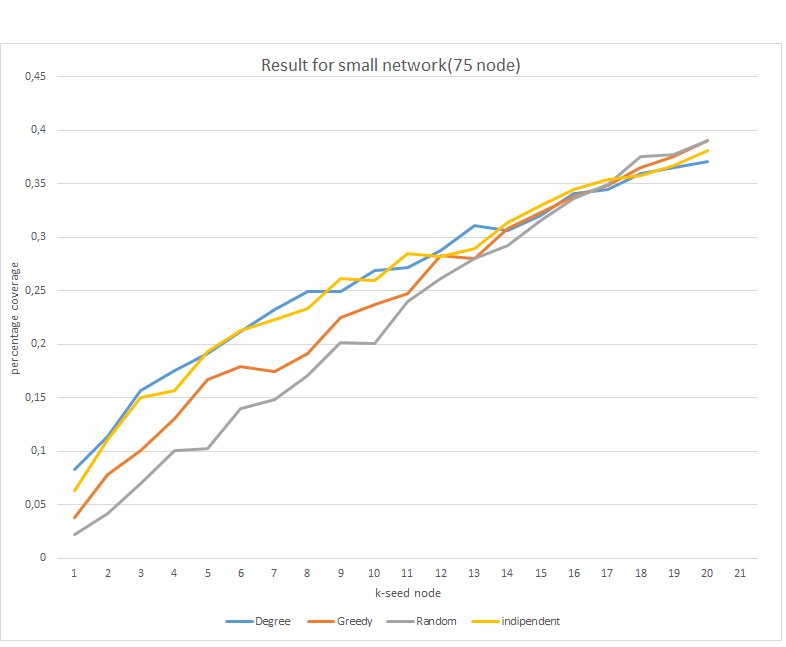
\includegraphics[width=\textwidth]{small_result}
	\caption{The result from the small graph} 
	\label{fig:smallResult}
\end{figure}



\begin{figure}
	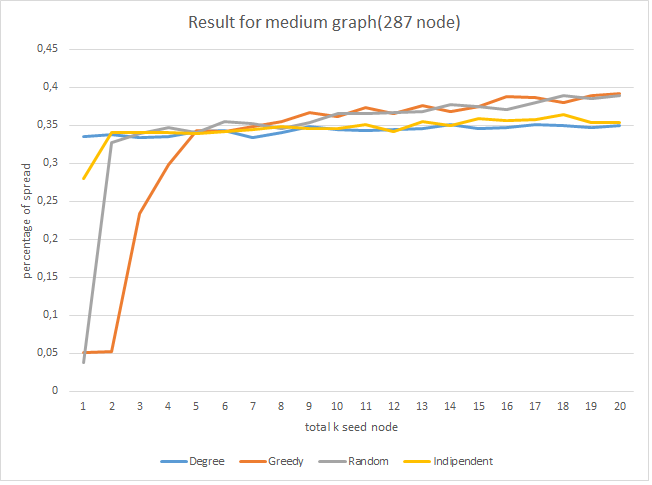
\includegraphics[width=\textwidth]{medium_result}
	\caption{The result from the medium graph} 
	\label{fig:mediumResult}
\end{figure}



\begin{figure}
	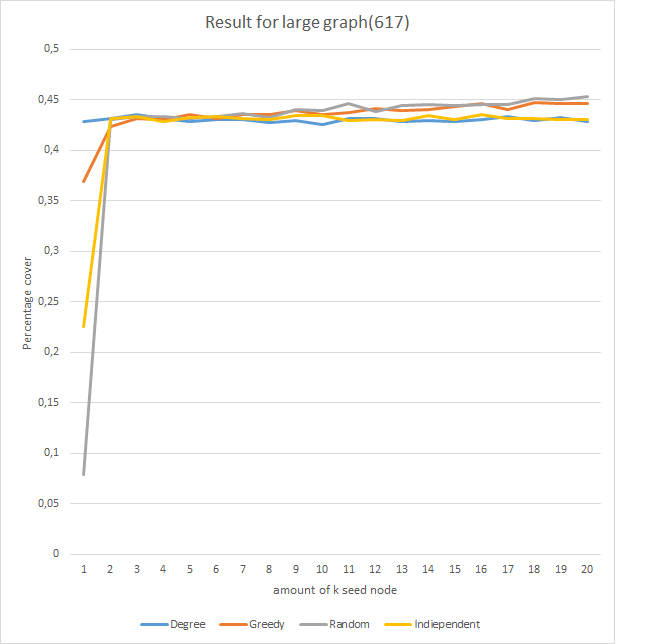
\includegraphics[width=\textwidth]{large_result}
	\caption{The result from the large graph} 
	\label{fig:LargeResult}
\end{figure}

We can see that the greedy algorithm performed better then the other algorithm for the large and medium graph, except the random algorithm for the large graph, where it was best.


